
% Chapter 2

\chapter{Research} % Main chapter title

\label{Chapter2} % For referencing the chapter elsewhere, use \ref{Chapter1} 

\lhead{Chapter 2. \emph{Research}} % This is for the header on each page - perhaps a shortened title

%----------------------------------------------------------------------------------------
%%%%%%%%%%%%%%%%%%%%%%%%%%%%%%%%%%%%%%%%%%%%%%%%%%%
%%%%%%%%%%%%%%%%%%%%%%%%%%%%%%%%%%%%%%%%%%%%%%%%%%%
%%%%%%%%%%%%%%%%%%%%%%%%%%%%%%%%%%%%%%%%%%%%%%%%%%%
\section{Case Studies}
This section examines a variety of schools---traditional and non-traditional, K-12 and post-secondary---to examine CS curriculum, benchmarks, pedagogy, course sequence, tools, and technologies. Independent schools with existing CS programs illustrate a path forward that may be closely aligned to Newman's own academic mission. Examining the top STEM public high schools (as ranked by the U.S. News in 2015), offers a vision of rigorous CS and engineering integration. The CS programs of both engineering and liberal arts colleges and universities shed light on post-secondary computer science, while an examination of code schools offers insight into an alternate approach to CS education. Finally, a review of local coding initiatives explains the state of coding in the region. Taken together, these examples place Newman's CS program in context both locally and nationally.
%----------------------------------------------------------------------------------------
%----------------------------------------------------------------------------------------
\subsection{Independent Schools}
\hiddensubsubsection{INDEX Schools} \label{index}
INDEX Schools is a collaboration of over 100 independent schools ``to share data, analysis, research, and information to aid member schools in decision-making, policy development, and strategic planning" \cite{index}. In early fall of 2016, nine schools responded to an INDEX listserv query requesting any curriculum outlines or standards and benchmarks for PK-12 computer science that schools might be willing to share. The results of the query are captured in a Google Spreadsheet: \href{http://bit.ly/1WFdwXN}{http://bit.ly/1WFdwXN}. \par 
Across the board, schools cited ISTE, CSTA, and AP benchmarks. Another salient trend is the use of \textit{physical computing}, the process of building programmable and interactive physical systems (e.g. robotics, Arduinos, Makey Makeys, etc.), in all divisions to make coding hands-on.   \par
The INDEX upper school programs are summarized in Table \ref{indexCS}. Almost all of the nine schools (8/9) who completed the survey offer the AP CS A course, although many schools are excited about the new AP CS Principles. All schools offered at least three tiers of CS, with most (7/9) offering 4 tiers. Three upper schools have graduation requirements, although several CS teachers hope to move towards a required credit. Greenhill has a one trimester requirement, Winchester Thurston requires two trimesters, and Porter-Gaud requires one semester. \par
A typical or traditional approach to CS (refer to Pingry, Park Tudor, and Ravenscroft) begins with an introductory CS course (typically in Java), followed by the AP, and concluding with advanced data structures or algorithms. Many schools, however, are beginning to adopt a much more creative approach to computer science that has broad applications to a myriad of disciplines. The course sequences of the four schools with the most innovative, thorough, and creative programs are listed in Table \ref{indexCScourses}. Winchester Thurston, as an example, offers an introductory CS series for humanities, art and music, or math/science, emphasizing the diverse applications of coding. All four of the schools summarized in Table \ref{indexCScourses} offer hands-on physical computing, in the form of robotics or XBox Kinect 3D body simulations. \par

\begin{table}[]
\centering
\caption{INDEX Upper School Summary}
\label{indexCS}
\begin{tabular}{|l|c|c|c|c|} \hline
\textbf{School}     & \textbf{Graduation Req.} & \textbf{AP} & \textbf{Physical Comp.} & \textbf{Tiers} \\ \hline
Fort Worth Country Day &                 & x  & x                  & 4     \\
Greenhill              & x               & x  & x                  & 4     \\
Lovett                 &                 & x  & x                  & 4     \\
Park Tudor             &                 & x  &                    & 4     \\
Pingry                 &                 & x  &                    & 3     \\
Porter-Gaud            & x               &    & x                  & 4     \\
Ravenscroft            &                 & x  &                    & 3     \\
St. Margaret's         &                 & x  &                    & 4     \\ 
Winchester Thurston    & x               & x  & x                  & 4     \\\hline
\textbf{TOTAL}		   & 3/9             & 8/9  & 5/9              & (4) 7/9 \\\hline
\end{tabular}
\end{table}
\begin{table}[]
\centering
\caption{Select Group of INDEX Upper School CS Programs}
\label{indexCScourses}
\begin{tabular}{|l|p{10cm}|} \hline
\textbf{School}     & \textbf{Program Summary} \\\hline

Greenhill & 				3 tiers, 2 year sequence \newline
							CS1: Introduction to CS with Arduino / Beginning JAVA Programming / Introduction to Game Design / Engineering \newline
							CS2: Advanced Computational Design / Intermediate JAVA Programming \newline
							CS3: Advanced Topics in Computer Science \\ \hline
Lovett &					Digital Media \& Interactive Design - animation, storytelling, 3D \& game design (1 semester) \newline
							CSI - Foundations (1 semester)\newline
							CSII - Media Computation \& App Development  (1 semester) \newline
							CSII - Robotics (1 semester) \newline
							APCS A - Java Programming (yearlong) \newline
							Honors Computer Science Studies (yearlong) \\ \hline
Porter-Gaud &				9th: Python Game Design, AppInventor App Design, Scribbler Robotics \newline
							10th: Web Design (HTML,CSS,PHP,SQL) \& C\#-XNA XBox Game Design \newline
							11th: Kinect 3D body simulations with C\#-XNA \newline
							12th: Java and iOS Swift \\ \hline
Winchester Thurston &		9 courses, 4 tiers \newline
							Level 1 - (1 trimester) CS for Humanities, CS for Art and Music, CS for Math/Science \newline
							Level 2 - AP CS, Software Structures, Physical Computing \newline
							Level 3 - CS Innovations (community involvement) \newline
							Level 4 - CS Innovations 2, Algorithm Design \\\hline

\end{tabular}
\end{table}
A summary of the middle school programs can be found in Table \ref{indexMS}. Seven of the nine schools interviewed offer CS in some form; all but one of these seven schools have a middle school CS requirement that is met either through integration into existing curriculum or through standalone elective courses. Computer literacy is not formally taught or itemized by the these INDEX schools. Like the upper school sequence, physical computing is a common theme; LEGO robotics and Arduinos are used in six of the nine programs that responded to the survey.\par
At the middle school level integration into existing curriculum is more prevalent than at the upper school level. At Lovett School in Atlanta, Georgia, integration occurs in 6th science through robotics, Scratch, and Arduino programming; in 7th and 8th grade, CS is offered as an elective. At Pingry School in New Jersey, all sixth graders take a co-curricular robotics class, and in 7th and 8th grade, a dedicated CS teacher integrates CS lessons into other classes.\par 
\begin{table}[]
\centering
\caption{INDEX Middle School CS Programs}
\label{indexMS}
\begin{tabular}{|l|p{2cm}|p{2cm}|p{2cm}|p{2cm}|p{2cm}|}\hline
\textbf{School} &	\textbf{Integrated}	& \textbf{Art/\newline Elective}	& \textbf{Physical Comp.} & \textbf{Required}	& \textbf{Years\newline Required}\\ \hline
FW Country Day &&&&	&0\\
Greenhill & &		x & 	x &	x &0.33\\
Lovett	& x &	x	& x	& x &0.25\\
Park Tudor &	& 	x &	 &&0		\\
Pingry	& x &  &			x &	x &0.25\\
Porter-Gaud	& &	x&	x &	x&0.5 \\
Ravenscroft	&&&&&0		\\
St. Margaret's & &		x &	x &	x&0.5\\ 
Winchester Thurston	& x  &	x &	x &	x&1\\\hline
\textbf{TOTAL}	& 3/9 &	6/9  &	6/9	& 6/9 &0.3(ave)\\\hline
\end{tabular}
\end{table}
Most of the schools interviewed in the survey (6/9) offer standalone CS courses as art electives. At Greenhill School in Dallas, Texas, all 5th and 6th grade students take ``Exploratory Design,'' a design thinking and engineering CS course that lasts one trimester and shares a elective block with another art credit (refer to the Greenhill section below for additional information). In 7th and 8th grade, CS courses at Greenhill are offered as fine arts electives. \par†
At St. Margaret's in San Juan Capistrano, CA, 6th and 7th graders take a quarter long required CS elective. At St. Margaret's there are seven blocks, five of which are core, one PE, and one elective; the  elective is comprised of 1/4 art, 1/4 music, 1/4 health \& wellness and 1/4 CS. The CS courses explore LEGO robotics, Arduinos, missions in Mindcraft, and Lua (through Codea). The 8th grade courses is a non-required semester-long elective in wearables, digital fabrication, programming, or art theater.\par
At Winchester Thurston in Pittsburgh, PA, there is a required, one-trimester elective each year of middle school, in addition to a maker elective. In 6th grade, the ``Create Year," students use Processing to draw pictures; in 7th, the ``Interact Year," students learn user interactions; and in 8th grade, ``Application Year," students use Arduinos to tie CS to other disciplines. \par
Of the middle school programs that responded to the INDEX query, the average CS requirement is equivalent to one trimester of CS throughout the middle school sequence. Winchester Thurston has the greatest requirement (one trimester each year, equating to one year throughout MS); St. Margaret's and Porter Gaud have two, quarter-long requirements; and Greenhill, Lovett, and Pingry have the equivalent of one quarter/ trimester CS course. \par
The lower school programs are summarized in Table \ref{indexLS}. One of the major trends across divisions and especially in primary education is the use of physical computing hardware (Bee-Bots, LEGO Robotics, Sphero, Makey Makey, etc.) to teach coding. At St. Margaret's students participate once a week in Imagine, Create, Engineer (ICE), hands-on exploration of design and innovation. Students in K-1 use Bee-Bots, programmable robots, to learn sequencing, logic, and math. Students also learn Scratch, and they develop these skills in 2nd - 5th grades. \par

\begin{table}[]
\centering
\caption{INDEX Lower School CS Programs}
\label{indexLS}
\begin{tabular}{|l|p{1.6cm}|p{1.6cm}|p{2cm}|p{2cm}|p{2.2cm}|}\hline
\textbf{School} & \textbf{Physical Comp.}& \textbf{Comp. Literacy}& \textbf{Integration}&\textbf{Standalone}&\textbf{Frequency}  \\ \hline
FW Country Day 	& x	
				& none					%computer literacy 
				&						%integration
				& x						%standalone
				& K-4: 1/week \\		%frequency
Greenhill 		& x
				& x						%computer literacy 
				&						%integration
				&x 						%standalone
				&2-4: 1/week		\\				%frequency
Lovett 			& x	
				& 						%computer literacy 
				&x						%integration
				& 						%standalone
				&K-5: Integr.		\\				%frequency
Park Tudor 		& x	
				& 						%computer literacy 
				&						%integration
				& 						%standalone
				&				\\		%frequency
Pingry 			& x
				&x 						%computer literacy 
				&						%integration
				&x						%standalone
				&K-5: 1/week			\\		%frequency
Porter-Gaud 	&
				& 						%computer literacy 
				&						%integration
				& 						%standalone
				&				\\		%frequency
Ravenscroft 	& x
				& 						%computer literacy 
				&						%integration
				& 						%standalone
				&none				\\		%frequency
St. Margaret's 	& x
				&x 						%computer literacy 
				&						%integration
				&x 						%standalone
				&K-5: 1/week					\\	%frequency 
Winchester Thurston & x
				& 						%computer literacy 
				&x						%integration
				& 						%standalone
				&K-5: Integr.			\\\hline	%frequency
\textbf{TOTAL}	& 8/9
				& 3/9						%computer literacy 
				& 2/9					%integration
				& 4/9					%standalone
				&  \\\hline				%frequency
\end{tabular}
\end{table}	
	
One of the primary questions that lower schools face is whether CS should be integrated into existing curriculum or taught as a standalone computer class. Although platforms like Scratch can be used in concert with any subject or curriculum, only two of the nine INDEX schools interviewed in this report integrate coding into other classes. The other major question facing lower school CS teachers is the role of coding vs. computer literacy. Although Greenhill currently blends computer science and computer literacy, Chris Bigenho, the Technology Director, believes that computer literacy should be left to classroom teachers. Mandy Lofquist at Fort Worth Country Day used to have a list of computer literacy benchmarks but has abandoned this list to make way for coding and making.\par
	
	
\hiddensubsubsection{Fort Worth Country Day School}
Fort Worth Country Day (FWCD) is an independent, coeducational K-12 school in Fort Worth, Texas with a total enrollment of over 1110. Three Newman faculty members toured the school in February of 2016 to observe their CS program. Their upper school CS sequence progresses as follows: 
\begin{itemize}
	\item 9th: Media Projects or AppInventor
	\item 10th: Art and Code with Processing
	\item 11th: AP CS A with Java
	\item 12th: Data Structures with Java
\end{itemize}
The US uses a block schedule. Classes meet for 75 minutes every other day for one semester. CS courses are treated as general electives, with the exception of “Art and Code,” which satisfies a fine arts credit. \par
There is no US CS requirement at FWCD. Media Projects is currently one section, there are two sections of Art and Code, one section of AP CS, and beginning next year, one section of data structures. With the exception of the introductory course, all CS classes are covered by one faculty member with a computer science background. \par
``Art and Code'' is a prime example of a course that emphasizes the creative capacity of coding. The course is taught in Processing, a visual programming language based on Java that is designed for artists. The teacher, Aaron Cadle, blends his own curriculum with content, labs, and projects developed by Darby Thompson, a CS teacher at Sidwell Friends School in Washington D.C. who has developed a project-based introductory CS course. During the observation, Aaron tested student’s understanding of abstract classes using a “Fish Tank” project. Students coded their own interactive, colorful fish that were placed on display in the library, and students outside of the course could vote on their favorite fish. \par
For AP CS Aaron relies on the \href{http://apluscompsci.com/}{A+ Computer Science curriculum}, which includes worksheets, labs, tests, slides, and notes. During the observation, students pulled personally-relevant datasets from data.gov (baseball stats, Powerball numbers, Hilary Clinton emails, etc.) and explored meaningful ways analyze the data using Java (e.g. finding the most common Powerball numbers). Aaron reversed the typical AP structure (lecture in class, worksheets for homework) in order to devote more time to workshopping labs. Students watch short (five minutes) instructional videos for homework and work on labs in class. \par
The upper-level CS course, Data Structures, is project based. The course is taught in Java and uses the XBox Kinect. Aaron uses the book, “Making Things See” by Greg Borenstein, which explores the use of Arduinos, Processing, and the Kinect to develop interactive programs. \par
As for middle school, coding exposure is currently limited to a two week HTML project that is integrated into 7th grade science. A newly hired middle school iPad coordinator, brought on to organize the division's one-to-one iPad program, is working to bolster computer literacy across campus. She currently uses 5th and 6th grade advisory time to teach digital citizenship, email etiquette, and Google Classroom. She is also developing curriculum for a required MS technology/computer literacy elective that may be offered next year. When asked about curriculum standards, she pointed to ISTE benchmarks. \par
Lower school computer science exposure at FWCD is very similar to Newman's. A ``Computer Special" offered to grades K-4 meets for 40 minutes every 1 out of 6 days. The class takes place in the ``lab"---a proto-makerspace/ design thinking workshopping space. The special explores engineering exercises, programmable hardware (Sphero, LittleBits, LEGO robotics, etc.), and coding (ScratchJr and Kodable). FWCD has never taught keyboarding; instead they direct interested parents/students to online resources. At one point the computer teacher, Mandy Lofquist, maintained a ``technology checklist" of all the computing skills her students should acquire, although she hasn't relied on this list since her students started coding. \par


\hiddensubsubsection{Greenhill School}
Greenhill School, a PK-12 coeducational private day school outside of Dallas, Texas, has an enrollment over 1200. This is another school that Newman faculty members toured in February, 2016 to observe their curriculum and classrooms. The Director of Technology, Chris Bigenho, has been researching computer science programs and developing K-12 CS curriculum for the last five years. Emphasis on aligning the program across divisions and with national standards, specifically CSTA, has led to the current implementation, which is one of the more advanced programs in the INDEX schools consortium. \par 
The upper school CS program is a three-tier, two year sequence. Students may take multiple courses from each tier (each a semester long course). There is a 1 trimester CS graduation requirement. The courses include:
\begin{itemize} 
	\item CS1: Introduction to CS with Arduino
	\item CS1: Beginning JAVA Programming 
	\item CS1: Introduction to Game Design 
	\item CS1: Engineering
	\item CS2: Advanced Computational Design
	\item CS2: Intermediate JAVA Programming
	\item CS3: Advanced Topics in Computer (prepares students for AP)
\end{itemize}
Greenhill’s middle school courses are broken into trimesters, and they rotate every 6 days. Classes meet for approximately 50 minutes. One block of the schedule is split between two electives; each meets every other day corresponding to ACE or BDF blocks. Band and choir may meet during ACE the entire year, while 2D or 3D art meets for a single semester during BDF. \par
Greenhill requires two trimesters of ``Exploratory Design,'' an elective that blends coding (Scratch, Arduino) with engineering design challenges. An example project includes prototyping, 3D printing, and testing a hub and blades for a wind turbine. The coding sequence is as follows:
\begin{itemize}
	\item 5th grade - Exploratory Design (required)
	\item 6th grade - Exploratory Design (required)
	\item 7th/8th grade - Prototyping 1 (optional elective)
	\item 7th/8th grade - Prototyping 2 (proposed optional elective)
	\item 7th/8th grade - Game Design (proposed optional elective)
\end{itemize}
Students may select additional maker or coding courses in 7th and 8th grade. Prototyping I is an optional arts elective that meets every other day for one trimester. Students work through ``Arduino Projects," a project book of 10+ exercises that introduce Arduino, servos, LEDs, and other simple circuits. \par
Now that Greenhill has an introductory CS course at the US level, the plan (discussed by both the MS head and the director of technology) is to consider making a CS course required in 7th and 8th grades. \par
The LS exposure takes place in 2nd - 4th grades in Computer 2, 3, and 4. These courses are a mix of computer literacy and coding (MicroWorlds), which is likely to change now that the computer teacher is retiring. Second grade students work on word processing, internet research, and educational computer games and apps. Second graders are introduced to coding with MicroWorlds EX. In addition to the skills and topics covered in second grade, third graders learn keyboarding and complete a six week coding project with MicroWorlds. In fourth grade students continue to explore previous subjects in computer literacy and coding in addition to learning file management and emailing. \par

\hiddensubsubsection{Nueva School}
The Nueva School is an independent, PK-12 school in Hillsborough and San Mateo, California, with an enrollment of over 700 students. Nueva is internationally-recognized ``for its distinctive inquiry-based interdisciplinary studies, constructivist project-based learning, and its pioneering work in social emotional learning and design thinking" \cite{nuevamis}. Design thinking, a human-centered and empathy-driven approach to solving problems, and engineering are heavily emphasized throughout and across divisions. IDEO and Stanford's d.School helped to develop the first PK-12 Design Thinking program and Innovation Lab (I-Lab).\par
The computer science program at Nueva is only two years old, but because design thinking and engineering are a core philosophy, Nueva's approach to computer science is unique. They currently don't align to any particular curriculum and believe the CSTA is too broad.\par 
In the upper school, CS is used as a problem-solving tool, rather than merely a standalone course, and is integrated into the mathematics and science curriculum. The mathematics department offers a course, ``The Elegant Logic of Computer Science," and beginning in grade 9, ``students grapple with age-old proofs, unlocking the power of computational programming on today's most robust platform to compile a digital portfolio demonstrating levels of mastery" \cite{nuevastem}. Students use Mathematica, a math-based programming language useful for solving integrals or plotting functions. Courses emphasize, among other things, computational thinking and ``integrated use of information technology" \cite{nuevastem}. \par
Another noteworthy upper school course, ``Technology \& Design Engineering," combines tools of a makerspace with engineering and design principles:
\begin{blockquote}
``A design innovation class, Design Thinking, Engineering \& Entrepreneurship empowers students to further build upon their skills developed in middle school to be change-makers in the world, helping them prepare for a future where resilience is key and translating ideas into reality, essential. Identifying needs and testing them, students generate ideas and create quick prototypes to get feedback, inventing business models to leverage their ideas in the world. Use of woodworking tools, CAD software, and digital fabrication equipment, such as the laser cutter and the 3-D printer, helps them bring their ideas to fruition" \cite{nuevastem}.
\end{blockquote}
Computer science is a tool for innovation and would strongly complement a course of this nature that emphasizes design thinking, engineering, and entrepreneurship.\par
The middle school program is still under development. There are no formal CS courses in 6th to 8th grade. Instead, smaller coding projects, such as animating infographics or presentations, are integrated into other core subjects.\par %castilleja
Lower school technology courses begin in second grade and continue through fifth grade (fifth grade is technically considered part of middle school). From their website: ``Lower school technology courses focus on introducing and developing emerging computing skills, including keyboarding, digital storytelling, conceptual programming, search and online research strategies, media literacy, ethical online behavior, and digital communication and collaboration skills" \cite{nuevalower}. The classes meet once a week for an hour in the Media Lab. According to their computer science director, the lower school is currently more of a technology course than a coding class, but moving forward, teachers will place greater emphasis on CS.
\begin{itemize}
	\item \textbf{2nd:} Keyboarding, basic word processing, learning about devices, and navigating the web. Multimedia projects and Scratch are creative outlets.   
	\item \textbf{3rd:} Keyboarding, email, Internet safety and ethics, research, organization, word processing, and the creation of communications for audiences other than oneself. Projects include Quicktime movies, Google Earth quests, and class blogs. Programming skills are reinforced with interactive Scratch projects. 
	\item \textbf{4th:} Keyboarding, using technology to communicate and collaborate, presentations, basic networking, saving to central servers, and file management. Projects include Quicktime movies, animations, and blog posts.\par
	\item \textbf{5th:} Internet research, organization, email/Internet safety and ethics, advanced word processing, spreadsheet creation and graphing, Scratch programming (iteration, conditionals, and variables).
\end{itemize}

%----------------------------------------------------------------------------------------
%----------------------------------------------------------------------------------------
\subsection{Public High Schools}
Examining the top fifteen STEM-ranked public high schools, as ranked by the U.S. News in 2015 \cite{usnews}, provides insight into the state of computer science in some of the nation's top science and engineering high schools. Roughly 3/4th of the list's top 15 schools offered at least one CS course, significantly more than the national average cited by Gallup of 1 in 4 U.S. schools \cite{gallup}. About half of these schools offered a basic (no requirement, strictly elective) computer science sequence: an introductory CS course (frequently in Java), followed by the AP CS course. Four of the 15 schools had a robust, scaffolded CS sequence; these schools are examined below. \par

\hiddensubsubsection{Thomas Jefferson High School for Science and Technology}
Thomas Jefferson High School for Science and Technology (TJ) is ranked \#2 on U.S. News' STEM report. A ``regional Governor's school" in Virginia with 1,846 enrolled students, TJ offers five years of Computer Science. There is a one credit CS graduation requirement that ``most students satisfy by taking Foundations of Computer Science in 9th grade during the summer" \cite{tjreq}. Additional courses (\href{https://www.tjhsst.edu/research-academics/math-cs/computer-science/docs/FlowCS1516.pdf}{the sequence for which can be found on their website}) include: AP Computer Science and Data Structures, Artificial Intelligence 1 \& 2, Parallel Computing 1 \& 2, Mobile App Development, Web App Development, and Mobile/Web Application Development Lab.\par
Thomas Jefferson HS's overall graduation requirements are listed in Table \ref{tjtable}. Computer science courses, including the graduation requirement, fall under ``electives." It is important to note that TJ's graduation requirements are largely similar to Newman's. \par
\begin{table}[]
\centering
\caption{Thomas Jefferson High School Graduation Requirements \cite{tjreq}}
\label{tjtable}
\begin{tabular}{lc}
\textbf{Subject}       & \textbf{Required Credits} \\ \hline
English                & 4                     \\
Math                   & 4                     \\
Science                & 4                     \\
History/Social Studies & 4                     \\
World Language         & 3                     \\
Health/PE              & 2                     \\
Fine Arts              & 1                     \\
Economics/Personal Finance              & 1                     \\ 
Electives              & 3                     \\
\textbf{Total}         & \textbf{26}          
\end{tabular}
\end{table}
\hiddensubsubsection{Stuyvesant High School}
Stuyvesant High School, a nationally-ranked New York City public high school with 3,285 students, ranked 14th on the U.S. News' top STEM schools. Stuyvesant offers 6 active CS courses that are listed through the math department. Although none of the CS courses satisfy the 4-sequence math requirement, students are required to take a single semester ``Introduction to Computer Science." In the introductory course, 
\begin{blockquote}``Students will study some the basic themes and subfields of computer science including algorithms and programming, simulation, networking, computability, graphics, and artificial intelligence. Students will also be given a solid foundation in working in a modern networked computer environment. This is a required course beginning with the Class of 2007. Students will take the course either in the Fall or Spring term of their sophomore year" \cite{stuy}.
\end{blockquote} 
Additional CS courses offered to high school students include: AP Computer Science, System Level Programming, Computer Graphics, Software Development, and Computer Science Intel Research. \par

\hiddensubsubsection{High Technology High School}
High Technology High School (HTHS) in Lincroft, New Jersey, has an enrollment of 280 and is ranked \#1 in U.S. News' top STEM schools. HTHS is relatively unique for its strong integration of technology and programming into engineering courses. CS courses include: Computer Programming for Engineers, Computer Science \& Software Engineering, and Digital Electronics \cite{hths}. \par

\hiddensubsubsection{Edison Academy for Science, Mathematics, and Engineering Technologies}
The Academy for Science, Mathematics, and Engineering Technologies, a magnet school located in Edison, New Jersey, has a total enrollment of 161 students and is ranked \#4 in the U.S. News top STEM public high schools \cite{usnews}. \par
The high school operates on a rotating block schedule; all classes meet Monday for one period, and classes meet on either Tuesday/Thursday or Wednesday/Friday for two periods (88 minutes). Engineering courses, however, meet every day of the week. Students enroll in either the ``civil and mechanical" or ``electronics and computer engineering" track. The requirements for the Electronics and Computer Engineering Technology (ECET) Program are listed in Table \ref{ecet}. \par
 \begin{table}[]
 \centering
 \caption{Edison Academy: Electronics and Computer Engineering Technology (ECET) Program of Study \cite{edisonacad}}
 \label{ecet}
 \begin{tabular}{|l|l|}
 \hline
 \multirow{4}{*}{9}  & Introduction to Engineering  \\ \cline{2-2} 
                     & Introduction to Digital Logic \\ \cline{2-2} 
                     & Introduction to Computer Science Using C++  \\ \cline{2-2} 
                     & DC Circuit Analysis \\ \hline
 \multirow{5}{*}{10} & Integrated Circuit Logic Families  \\ \cline{2-2} 
                     & Sequential Logic Circuits \\ \cline{2-2} 
                     & Finite State Machines (FSM) \\ \cline{2-2} 
                     & Interfacing to the analog world \\ \cline{2-2} 
                     & Microcontrollers / Assembly language \\ \hline
 \multirow{4}{*}{11} & Object Oriented Programming Using C++  \\ \cline{2-2} 
                     & AC Circuit Analysis \\ \cline{2-2} 
                     & Electronic Communication Systems \\ \cline{2-2} 
                     & Digital Communication Systems \\ \hline
 \multirow{2}{*}{12} & Senior Project \\ \cline{2-2} 
                     & Programming with JAVA \\ \hline
 \end{tabular}
 \end{table}
 %---------------------
\hiddensubsubsection{Westside Magnet High School for Integrated Technology}
Although Westside Magnet High School for Integrated Technology, did not make U.S. News' list of top 15 public STEM schools, its robust CS program warrants attention. The magnet school in Houston, Texas gives students the option to choose one of five magnet strands in business, computing sciences and engineering, fine arts, health science and technology, or media. Students take strand-specific courses during the ``magnet'' elective block (highlighted in orange in Table \ref{westsidesched}). Students who choose the ``Computing Sciences and Engineering" select between one of three programs: Computer Programming, Computer Maintenance, and Engineering. The courses comprising these programs are outlined in Table \ref{westsidemag}. The school reportedly uses the four year engineering curriculum developed by \href{https://www.pltw.org/}{Project Lead the Way} \cite{westside}.
\begin{table}[]
\centering
\caption{Four Year Plan for Westside HS Computing Sciences and Engineering \cite{westside}}
\label{westsidesched}
\begin{tabular}{|l|l|l|l|}
	 \hline
\textbf{9th}     & \textbf{10th}        & \textbf{11th}         & \textbf{12th}               \\ \hline
English          & English              & AP Language           & AP Literature               \\ \hline
Algebra/Geometry & Geometry/ Algebra II & Alga. II/Pre-Calculus & Pre-Calculus/Calculus       \\ \hline
World Geography/ & World History        & U S History           & Go/Economics                \\ \hline
Biology          & Chemistry            & Physics               & AP Science/Elective Science \\ \hline
Foreign Language & Foreign Language     & Foreign Language      & Health/Speech               \\ \hline
\rowcolor[HTML]{FFCC67} Magnet Course   & Magnet Course        & Magnet Course         & Magnet Course   \\ \hline
Fine Arts Credit & PE                   & Elective              & Elective					  \\ \hline                   
\end{tabular}
\end{table}


\begin{table}[]
	\centering
	\footnotesize
	\caption{Westside HS Computing Sciences and Engineering Magnet Courses \cite{westside}}
	\label{westsidemag}
	\begin{tabular}{|p{2cm}|p{3.1cm}|p{3.1cm}|p{3.1cm}|p{3.1cm}|p{3.1cm}|}
		\hline
	\textbf{Program} & \textbf{9th}     & \textbf{10th}        & \textbf{11th}         & \textbf{12th}               \\ \hline
Computer Programming & Principles of Information Technology/ Principles of Art, A/V Technology and Communication & Pre-AP Computer Science 1 (Python) or Computer Programming & Pre-AP Computer Science 2 (JAVA) or Pre-AP Computer Science 1 (Python) & AP Computer Science 1 (JAVA) or Pre-AP Computer Science 2 (JAVA) \\ \hline
Computer Maintenance & Principles of Information Technology/ Principles of Art, A/V Technology and Communication & Computer Maintenance & Telecommunications and Networking & Research and IT Solutions or Practicum in Business Management    \\\hline
Engineering Design & Introduction to engineering Design & Principles of Engineering & Digital Electronics & Engineering Drafting and Design \\\hline
Engineering Practice & Concepts of Engineering & Robotics & Principles of Technology & Engineering Mathematics \\ \hline                                    \end{tabular}
\end{table}

%----------------------------------------------------------------------------------------
%----------------------------------------------------------------------------------------
\subsection{Higher Education}
Preparation for college is obviously paramount in any upper school academic program at Newman, and so it's instructive to examine the range of CS courses and subjects offered in higher education. \par
\hiddensubsubsection{MIT}
Massachusetts Institute for Technology (MIT) is a consistently top-ranked, globally-recognized leader in education, research, and innovation. MIT's Electrical Engineering and Computer Science (EECS) Department is the largest department at MIT and is composed of four undergraduate degree programs: Electrical Science and Engineering, Electrical Eng. \& Computer Science, Computer Science and Engineering, and Computer Science and Molecular Biology. All four tracks are required to take EECS I, an introductory electrical engineering and computer science course:
\begin{blockquote}
\textbf{6.01 Introduction to EECS I} - An integrated introduction to electrical engineering and computer science, taught using substantial laboratory experiments with mobile robots. Key issues in the design of engineered artifacts operating in the natural world: measuring and modeling system behaviors; assessing errors in sensors and effectors; specifying tasks; designing solutions based on analytical and computational models; planning, executing, and evaluating experimental tests of performance; refining models and designs. Issues addressed in the context of computer programs, control systems, probabilistic inference problems, circuits and transducers, which all play important roles in achieving robust operation of a large variety of engineered systems \cite{mit}.
\end{blockquote}
There is a close link between electrical engineering and computer science throughout MIT's undergraduate CS program. Thanks to tools like Arduinos, Raspberry Pis, VEX and LEGO robotics, and other easily-programmed microcontrollers, it's possible to develop upper school curriculum that explores computer science through an electrical or mechanical engineering lens. As for CS fundamentals, MIT's more traditional introductory CS course is described below:
\begin{blockquote}
	\textbf{6.S04 Special Subject: Fundamentals of Programming} - Introduces fundamental concepts of programming. Designed to develop skills in applying basic methods from programming languages to abstract problems. Topics include programming and Python basics, computational concepts, software engineering, algorithmic techniques, data types, and recursion and tail recursion. Lab component will consist of software design, construction and implementation of design \cite{mit}. 
	\end{blockquote} \par

\hiddensubsubsection{Pomona College}
Pomona College, a small liberal arts college in Claremont, California, offers the perspective of a top-tier, post-secondary school without an engineering department. CSCI051 is the first course in the CS sequence, and it specifies that no previous programming experience is required.
\begin{blockquote}
	\textbf{CSI051} - Introduction to the field of computer science using the object-oriented language Java. Topics include iteration and recursion, basic data structures, sorting and searching, elementary analysis of algorithms and a thorough introduction to object-oriented programming. Special emphasis on graphics, animation, event-driven programming and the use of concurrency to make more interesting programs  \cite{pomonacs1}. 
\end{blockquote}
CSCI052, the second course in the introductory series, emphasizes ``functional programming, procedural and data abstraction, recursion and problem-solving" as well as ``computer architecture and organization, finite automata and computability" \cite{pomonacs1}. These subjects are closely aligned with the CSTA benchmarks for upper level computer science.  \par 

%----------------------------------------------------------------------------------------
%----------------------------------------------------------------------------------------
\subsection{Code Schools}
Around the country code schools are emerging in response to the growing need for software engineers, a need that is not being met by colleges and universities. Code schools are akin to traditional trade schools; employment is the primary focus, and career placement drives the curriculum. For that reason, code schools offer a different approach to computer science than traditional education. Some of the differences may include: strong emphasis on project-based learning, web development languages (JavaScript, Ruby, etc.), greater emphasis on applied rather than theoretical CS, group collaboration using Git and version control, portfolio creation, and interview preparedness. \par 
\href{http://www.hackreactor.com/curriculum}{Hack Reactor} is perhaps one of the most well-known and rigorous code schools. Their website states that ``students build apps from the ground up and start businesses before they are even out of the program" \cite{hackre}. Their website showcases projects like drones, Android fitness role playing games, web data visualizations, and more. According to Ian deBoisblanc, a Hack Reactor student in San Francisco, the program is mostly project-oriented and has three overarching themes: learning how to learn, learning by doing, and learning how to work together (Git workflow). The course covers foundational CS topics: algorithms, Big-O notation, functional programming, recursion, data structures, a little bit of networks and computer architecture, classes, polymorphism, APIs, and lots of HTML and CSS. Students also spend an extended period of time on a project they take over from another student, emphasizing the need to write code that is organized and human-readable. Finally, they work on a mini `thesis' as the capstone of the experience.\par
Operation Spark, detailed in the next section \cite{opspark}, is a local example of a code school. Like Hack Reactor, they use JavaScript, and explore web design, functional and object-oriented programming, and portfolio development.\par
On the CS educational spectrum, code schools could be considered at the applied, `concrete' end, while theoretical, academic computer science taught or employed in universities might represent the other end of the spectrum. K-12 education needs to find its place in this continuum by identifying and articulating its own academic mission. Is the objective to prepare students for college, to graduate students who are ready for coding employment, or to merely give students a flavor of the diverse applications of CS? The answer is likely a blend of the above, and straddling the pedagogical approaches is the best way to prepare students for a variety of future experiences in computer science.\par

%----------------------------------------------------------------------------------------
%----------------------------------------------------------------------------------------
\subsection{Local Initiatives}
%TODO local schools
\hiddensubsubsection{Independent Schools}
Metairie Park Country Day School (MPCDS) is currently in a similar boat as Newman. MPCDS currently offers an introductory and AP CS course in the upper school. Teachers in the middle school are exploring ways to integrate Scratch and Arduinos into the curriculum. Several teachers have also taken an Arduino course as a means to explore the possibility of physical computing.\par
According to the Tech Director at McGehee School, Margaret Ann Minihan, McGehee currently offers some computer science in grades 3-12. Flor Serna, the founder of \href{http://www.electricgirls.org/}{Electric Girls}, taught coding, making, wearable tech, and electronics to middle school students using tools like Arduinos and Makey Makeys. Beginning next year, however, Flor will be teaching at St. Martin's, another independent school in the region with a standout making and coding curriculum. 

\hiddensubsubsection{Public/ Charter Schools}
Benjamin Franklin High School currently offers CS as an elective. This year there is one section of AP Computer Science and two sections of Introduction to Computer Science that has mostly 9th graders. According to the CS teacher, the Intro course is a collection of exercises from the internet or created in-house. Topics include (limited) programming, two-wheeled robot programming, Raspberry Pi coding, a paper on a controversial topic related to CS, basic Excel skills, Photoshop/Illustrator/InDesign, and some beginning cryptography and security.\par

Lusher Charter High School is currently offering engineering and computer science electives using the \href{https://www.pltw.org/}{Project Lead the Way} curriculum. ``Computer Science Principles" serves as the introductory computer science course and is aligned with the AP CS Principles. The CS and engineering courses include \cite{lusherhigh}:
\begin{itemize}
	\item Introduction to Engineering (1 year, 1 unit): This course offers ``hands-on opportunities for students to develop technical solutions to meet real world needs using 3-dimensional computer aided design software to develop models and create hardware based on their models.''
	\item Principles of Engineering (1 year, 1 unit): ``This survey course uses 3D modeling software and VEX robotics equipment...Topics include mechanisms, energy, statics, materials, and kinematics. Pre-req: Introduction to Engineering"
	\item Computer Science and Software Engineering (1 year, 1 unit): ``Students create apps for mobile devices, automate tasks in a
variety of languages, and find patterns in data. Students collaborate to create and present solutions that can improve people’s lives, and weigh the ethical and societal issues of how computing and connectivity are changing the world. This course aligns with the AP Computer Science Principles course."
	\item Engineering Level IV - Design and Development (1 year, 1 unit): ``Engineering Design and Development (EDD) is the capstone course in the PLTW high school engineering program. It is an engineering research course in which students work in teams to design and develop an original solution to a valid open-ended technical problem by applying the engineering design process."
\end{itemize}

\hiddensubsubsection{Alternative Programs}
\href{http://www.nolacode.org/}{NOLA Code} is an after school K-8 program targeting public/charter schools. The program is free to students on free/reduced lunch. NOLA Code introduces programming using Scratch and Code.org exercises.\par
\label{opsp}\href{https://operationspark.org/}{Operation Spark} is a non-profit that hopes to combat generational poverty by offering software engineering training to low-income, out of school, and unemployed youth in New Orleans. They also offer a limited number of seats for paying applicants to participate in their coding bootcamp. Their website outlines the skills covered in this program \cite{opspark}:\par
Fundamentals of Computing, HTML, CSS and JS
\begin{itemize}
	\item Understanding Hardware, OS, applications, data, and the file system
	\item Terminal Basics: pwd, ls, cd, mkdir, touch
	\item Markdown: interpreting markup languages
	\item HTML: Structure, Text, Lists, Tables, Images, Links, Forms
	\item CSS Styling: Colors, Text, Boxes
	\item CSS Positioning: responsive/mobile, grids, frameworks
	\item Git Fundamentals: clone, add, commit, push
	\item JS Fundamentals: values, operators, flow control, loops, arrays, objects,functions
\end{itemize}
Functional JavaScript
\begin{itemize}
	\item Functional JS (underscore): reimplement each, map, first, last, shuffle, contains, filter/select, every, any
	\item JavaScript in the browser environment (DOM interface, localStorage, window, events, Ajax) \& jQuery
	\item Advanced HTML: video, audio, canvas, data attributes
	\item Simple design patterns \& micro-utilities: module pattern (for creating private vars), a testing library, a dependency injection system, eventing library, templating library 
\end{itemize}
Object Oriented JavaScript
\begin{itemize}
	\item OO JS: just decorator pattern, functional instantiation, Object.create
	\item Using Chrome Developer Tools
\end{itemize}
Job Skills \& Building a Portfolio Site
\begin{itemize}
	\item Advanced Implementations
	\item Using Google Maps, Stripe, Soundcloud \& other 3rd party API’s
	\item Brief introduction to using Backend-as-a-Service (Parse, Firebase)
\end{itemize}

%%%%%%%%%%%%%%%%%%%%%%%%%%%%%%%%%%%%%%%%%%%%%%%%%%%
%%%%%%%%%%%%%%%%%%%%%%%%%%%%%%%%%%%%%%%%%%%%%%%%%%%
%%%%%%%%%%%%%%%%%%%%%%%%%%%%%%%%%%%%%%%%%%%%%%%%%%%
\section{National Standards}

%----------------------------------------------------------------------------------------
%----------------------------------------------------------------------------------------
\subsection{Computer Science Teachers Association}
The Computer Science Teachers Association (CSTA) released the revised ``K-12 Computer Science Standards" in 2011, which is widely cited in the computer science education community as a source of CS benchmarks. The CSTA outlines a set of learning objectives on three levels and grouped into one of five ``strands": computational thinking; collaboration; computing practice; computers and communication devices; and community, global, and ethical impacts \cite{csta}. The benchmarks begin at the elementary level and continue through high school. AP CS curriculum fits well into the level 3 CSTA sequence, but CSTA recommends additional CS courses for depth. For the list of standards, refer to Appendix \ref{AppendixCSTA}.\par


%----------------------------------------------------------------------------------------
%----------------------------------------------------------------------------------------
\subsection{International Society for Technology in Education}
The International Society for Technology in Education (ISTE) has compiled a set of standards for computer science educators \cite{iste}. These standards are listed in Appendix \ref{AppendixISTE} and are cross-referenced with CSTA benchmarks. Unlike CSTA, ISTE does not describe K-12 standards, but rather outlines a set of learning objectives that could presumably be covered in one or more advanced high school courses. When mapped to the CSTA benchmarks, ISTE standards mostly fall under level 3A (at the AP CS level) are are not particularly useful for identifying the requirements for introductory curriculum. In addition to computer science concepts, these standards layout teaching standards and strategies specific to educators and learning environments. \par


%----------------------------------------------------------------------------------------
%----------------------------------------------------------------------------------------
\subsection{Computing at School}
Computing at School (CAS) is a community of computer science educators and industry professionals with over 150 regional hubs in the United Kingdom. This community is passionate about computer science education, and in 2012, CAS published a set of standards titled, ``Computer Science: a Curriculum for Schools'' \cite{computas}, which are listed in Appendix \ref{AppendixCOMP}.\par 
CAS breaks the standards into five subject areas: algorithms, programs, data, computers, and communication \&internet. These benchmarks are broken into ``Key Stages'':
\begin{itemize}
	\item Key Stage 1 (K-2nd)
	\item Key Stage 2 (2nd-5th)
	\item Key Stage 3 (5th-9th)
	\item Key Stage 4 (9th-12th)
	\item Post K-12 education
\end{itemize}

%----------------------------------------------------------------------------------------
%----------------------------------------------------------------------------------------
\subsection{College Board's Advanced Placement}
\label{CBAP}Since 2003 the \href{http://media.collegeboard.com/digitalServices/pdf/ap/ap-course-overviews/ap-computer-science-a-course-overview.pdf}{Advanced Placement Computer Science A} exam has tested students' ability to solve problems and design algorithms using Java. The College Board's test is intended to cover the equivalent of a first semester college computer science course. The topics include:
\begin{enumerate}
	\item Object-Oriented Program Design:  Program and class design 
	\item Program Implementation: Implementation techniques. Programming constructs, Java library classes
	\item Program Analysis: Testing, Debugging, Runtime exceptions, Program correctness, Algorithm analysis
	\item Standard Data Structures:  Primitive data types, Strings, Classes, Lists, Arrays (1-D and 2-D) 
	\item Standard Operations and Algorithms: Searching, Sorting
	\item Computing in Context: System reliability, Privacy, Legal issues and intellectual property, Social and ethical ramifications of computer use 
\end{enumerate}
In 2016 the College Board plans to release a second AP CS course, \href{https://secure-media.collegeboard.org/digitalServices/pdf/ap/ap-computer-science-principles-curriculum-framework.pdf}{AP Computer Science Principles}, that will operate in tandem to the other AP CS class. From the AP website, ``AP Computer Science Principles offers a multidisciplinary approach to teaching the underlying principles of computation." Unlike the AP CS A which relies exclusively on Java, the Principles course allows teachers to use any programming language. The course introduces key programming concepts with a ``focus on fostering students to be creative." The ``Big Ideas" covered by this exam include:
\begin{enumerate}
	\item Creativity
	\item Abstraction
	\item Data and Information
	\item Algorithms
	\item Programming
	\item Internet
	\item Global Impact
\end{enumerate} \par
\begin{table}
	\centering
	\bgroup
	\def\arraystretch{1.5}
	\begin{tabular}{ p{7cm} p{7cm} }
		\hline
		\textbf{AP Computer Science \textit{A}} &	\textbf{AP Computer Science \textit{Principles}} \\ \hline \hline
		\multicolumn{2}{l}{\textit{Curriculum:}} \\
		Focused on object-oriented programming and problem solving & Built around fundamentals of computing including problem solving, working with data, understanding the Internet, cybersecurity, and programming. \\ \hline
		\multicolumn{2}{l}{\textit{Language:}} \\
		Java is the designated programming language	& Teachers choose the programming language(s) \\ \hline
		\multicolumn{2}{l}{\textit{Skillset:}} \\
		Encourages skill development among students considering a career in computer science or other STEM fields & Encourages a broader participation in the study of computer science and other STEM fields, including AP Computer Science A \\ \hline
		\multicolumn{2}{l}{\textit{Assessment:}} \\
		Multiple-choice and free-response questions (written exam) & Two performance tasks students complete during the course to demonstrate the skills they have developed (administered by the teacher; students submit digital artifacts), and multiple-choice questions (written exam) \\ \hline
	\end{tabular}
	\egroup 
	\caption{Comparison of AP Computer Science Exams ~\cite{APcomp}} \label{tab:apexams} 
\end{table}\par
For a detailed list of learning benchmarks associated with this exam, \href{https://secure-media.collegeboard.org/digitalServices/pdf/ap/ap-computer-science-principles-curriculum-framework.pdf}{check out the AP Computer Science Principles Curriculum Framework}. \par

\hiddensubsubsection{Pros \& Cons of AP CS} \label{proconap}
There are merits and shortcomings of teaching Advanced Placement courses in general, as well as those that are specific to computer science. Perhaps the most salient advantage is the potential for college credit, which may allow students to place out of introductory-level college courses and save time or money in higher education. AP courses may also positively affect college transcripts since AP courses at Newman are weighted in the student’s cumulative GPA calculation. In addition, because College Board is an internationally-recognized organization, there is a thriving community willing to offer support or share resources, curriculum, example labs, and exercises. Finally, the AP course offers a set of well-researched standards and benchmarks that, at in theory, align with equivalent college-level courses. \par
Perhaps one of the greatest criticisms of AP courses in general is the rigidity and inflexibility of the curriculum. John Tierney, a contributing writer for The Atlantic and a former professor of American government at Boston College, writes:
\begin{blockquote}
	``In short, AP courses are a forced march through a preordained subject, leaving no time for a high-school teacher to take her or his students down some path of mutual interest. The AP classroom is where intellectual curiosity goes to die" \cite{atlantic}.
	\end{blockquote}
This shortcoming is particularly stifling and problematic in AP CS A. Given the substantial amount of theory and subject matter covered on the exam, the course affords little opportunity for project-based, open-ended discovery and expression. The AP CS A course requires Java, a language that comes with significant paradigm baggage, and limits students to the kinds of programming that can be expressed with Java. Although Java is a common language in introductory college courses, the most common teaching language at the university level as of July, 2014 is Python \cite{unilang}, a language that allows students ``to focus less on details such as types, compilers, and writing boilerplate code and more on the algorithms and data structures relevant to performing their intended tasks" \cite{guo}. And although the curriculum provides a sound introduction to the theory and mindsets of CS, the AP CS A exam renders an infinitely creative subject into a formulaic and uninventive practice, which is not the most effective approach for engaging and capturing a diverse group of students. \par 
The AP CS Principles course has the potential to mitigate many of these criticisms. The course website states that the impetus for developing the course was the need to ``increase the number of students interested in and prepared for success in computer science and other STEM fields'' \cite{apcsfaq}. The course does not specify a specific programming language, but instead encourages students to develop ``personally relevant artifacts'' \cite{apframe}, whether these are web apps, digital music, animations, or mobile games. ``The course is unique in its focus on fostering students to be \textbf{creative}'' \cite{apframe} (the use of bold font to emphasize ``creative'' comes straight from the document).  There is also greater emphasis on appealing to a broader audience by highlighting the impacts of computational thinking on a myriad of fields, not just computer science. \par

On paper the new AP CS Principles course is the answer to the need for a college-level, nationally-recognized CS course that doesn't stifle innovation, creativity, and personalized, project-based learning. The course, however, is still young, and it may take time to answer questions such as, how will colleges respond? Is this course sufficiently rigorous preparation for college-level CS? Do the curriculum and benchmarks still afford space for creativity and exploration? Will students, particularly those from underrepresented groups, feel more inclined to take this new AP course? \par
 
As for enrollment, it's unclear how the AP designation might affect course registration at Newman. The AP CS Principles states that ``students do not need to have prior knowledge of any programming language'' \cite{apcsfaq}. Offering an AP as the introductory course may deter students who are unfamiliar with CS, particularly its creative dimension, from signing up for a rigorous course. Even if AP CS Principles is the second or third course in the CS series, there may be unpredictable impacts on registration. For example, high-achieving students who might typically take AP Biology or Chemistry electives may be more likely to take AP CS since it would offer the same GPA and transcript distinctions as other AP science or math courses, while students with a passion for computer science but who desire a less rigorous course load might shy away from an AP CS course. Another alternative---offering an AP caliber course that prepares students for an optional AP exam at the end of the semester---may cater to both groups of students. Ultimately, student feedback is necessary to determine the best course of action to maximize enrollment. \par


%----------------------------------------------------------------------------------------
%----------------------------------------------------------------------------------------
\iffalse\subsection{Next Generation Science Standards}
The Next Generation Science Standards (NGSS) is the product of twenty-six states and broad-based teams working to develop a new set of science standards needed to revise a 15-year-old set of documents on which most state standards are based \cite{ngsss}. Unfortunately, the latest NGSS document does not enumerate standards specific to computer science, for the reasons explained below:
\begin{blockquote}
``Computer Science and Statistics Computer science and statistics are other areas of science that are not addressed here, even though they have a valid presence in K-12 education... Computer science, too, can be seen as a branch of the mathematical sciences, as well as having some elements of engineering. But, again, because this area of the curriculum has a history and a teaching corps that are generally distinct from those of the sciences, the committee has not taken this domain as part of our charge. Once again, this omission should not be interpreted to mean that computer science or statistics should be excluded from the K-12 curriculum. There are aspects of computational and statistical thinking that must be understood and applied in learning about the sciences, and we identify these aspects, along with mathematical thinking, in our discussion of science practices in Chapter 3" \cite{ngsss}. 
\end{blockquote}\par
Although the NGSS does not explicitly outline CS benchmarks, the Engineering Design standards are highly applicable to software engineering or computational thinking projects. These benchmarks are covered in Appendix \ref{AppendixNGSS}. \par
For CS courses that are not standalone but rather are integrated into existing math or science classes, aligning curriculum with relevant NGSS standards may be advisable. Code.org has published two sets of middle school curriculum---CS in Algebra and CS in Science---that are consistent with both CSTA and NGSS standards. A table summarizing the overlap between these standards as it relates to this curriculum can be \href{https://code.org/curriculum/science}{found on their website}.\fi

%%%%%%%%%%%%%%%%%%%%%%%%%%%%%%%%%%%%%%%%%%%%%%%%%%%
%%%%%%%%%%%%%%%%%%%%%%%%%%%%%%%%%%%%%%%%%%%%%%%%%%%
%%%%%%%%%%%%%%%%%%%%%%%%%%%%%%%%%%%%%%%%%%%%%%%%%%%
\section{Online Curriculum}
A non-exhaustive list of online coding tools and curriculum can be found in Appendix \ref{AppendixTools}. Tools are separated by level (lower, middle, and upper school). The table contains information about professional development, platform cost, student tracking, and the possibility for self-guided online learning. \par 
At the elementary school level, iPad apps (Kodable) and drag-and-drop visual programming languages (Hopscotch, Scratch, SNAP!, Tynker) teach foundational coding concepts through interactive games, art, and animations. Many of these platforms cater to teachers without computer science experience. For example, Tynker includes assessment, classroom management, lesson plans, and a built in tutor. In addition, Tynker aligns to Common Core Mathematics, Common Core ELA, and CSTA Computer Science standards \cite{tynker}. \par
Many of the elementary-level tools (Scratch, Tynker, SNAP!) can be used in more sophisticated projects at the middle school level. For integrating CS into existing middle school courses, Code.org provides 20-lesson CS in Algebra and CS in Science modules, as well as in-person or online professional development. \par

\hiddensubsection{Massive Open Online Courses}
There is great diversity in the number of online courses available to upper school students thanks to the rise of massive open online courses MOOCs. A multitude of computer science courses and subjects can be found on sites such as Coursera, Udemy, Kahn Academy, Udacity, edX, and others. Only a few, however, are optimized for high school instruction and include student tracking, rigorous assessments, standards and benchmarks, or content structured for a typical upper school schedule. The relevant platforms are explored below. \par
\hiddensubsubsection{Kahn Academy} 
Kahn Academy offers two ``computing'' tracks: computer programming and computer science. The former uses Processing.js and JavaScript to cover the following topics (in order): basic statement syntax, variables, math operators, assignment operators, strings, functions, logic and conditionals, loops, arrays, objects, and object-oriented JS. Student tracking is possible through the teacher backend. The courses include 40 talk-throughs, 35 challenges, and 10 projects, which reportedly comes out to about 15 hours of curriculum \cite{kahnresource}.  The modules include:
\begin{itemize}
	\item Intro to JS: Drawing \& Animation
	\item Intro to HTML/CSS: Making webpages
	\item Intro to SQL: Querying and managing data
	\item Advanced JS: Games \& Visualizations
	\item Advanced JS: Natural Simulations
	\item HTML/JS: Making webpages interactive
	\item HTML/JS: Making webpages interactive with jQuery
	\item Meet the professional
\end{itemize}
Kahn Academy's ``computer science'' track includes modules in algorithms, cryptography, information theory, and the internet, all of which require an understanding of CS coding fundamentals. Taken with the computer programming track, Kahn Academy could offer a possible source for self-guided instruction at Newman. \par

\hiddensubsubsection{Codeacademy} 
Codeacademy is very similar to Kahn Academy in assessment and content, and students are immediately creating web visualizations or content in the browser. One difference is Codeacademy's click-through instructional style, which may feel more cumbersome than the video instruction offered by Kahn Academy. Units take approximately 8 hours to complete and include:
\begin{enumerate}
	\item Web Fundamentals - HTML/CSS (20 lessons)
	\item Python (36 lessons)
	\item JavaScript (28 lessons)
	\item jQuery (6 lessons)
	\item PHP (11 lessons)
	\item Make a Website (5 lessons)
	\item Make an Interactive Website (9 lessons)
	\item Ruby (30 lessons)
\end{enumerate}
While Codeacademy and Kahn Academy offer student tracking and a diversity of topics, online schools such as CodeHS, Edhesive, and Global Online Academy simulate the experiences of rigorous, in-class instruction aligned to nationally-recognized benchmarks. \textbf{Global Online Academy} \label{oga} currently offers self-motivated Newman students the ability to take the following CS courses:
% http://www.globalonlineacademy.org/the-goa-experience/courses/
\begin{itemize}
\item Art of Code: Processing
\item Computer Programming I: Computational Thinking
\item Computer Programming I: Java
\item Computer Programming II: Advanced Java
\item Computer Programming II: Analyzing Data with Python
\item Computer Programming II: iOS Development
\end{itemize}
For a small number of students, Global Online Academy is a cost effective---\$500 per student per semester---solution to offering limited CS exposure. This platform, however, is not scalable as a solution to meet a possible CS graduation requirement. Beyond a single section, the courses are no longer cost effective, in addition to the fact that registering more than 2-4 students is likely impossible due to competition from other schools.\par
\hiddensubsubsection{Edhesive} 
Edheisve is an online platform optimized to help upper school teachers and administrators get CS programs off the ground. From their promotional materials, ``Our program is an all-in-one blended online solution that enables a school to provide Intro and AP Computer Science to its students, even without an AP CS teacher on staff. It includes College Board-approved curriculum with video lessons, automatically-graded assessments, and an active, online forum for content support.'' Edhesive relies on in-class ``coaches'' who primarily serve an administrative role. Students get support 7 days/week in an online forum monitored by the online course instructor and TAs. The program appears to be effective. Edhesive boasts of a class average a 3.3 on the 2014 AP CS Exam, while the national average was a 2.95.\par

\hiddensubsubsection{CodeHS} 
CodeHS is perhaps the closest competitor to Edhesive. CodeHS offers three courses: Intro to CS, AP CS Principles, and AP CS A. Like Kahn Academy and Codeacademy, CodeHS uses in-browser code-able animations and games (Karel and JavaScript); however, CodeHS is designed specifically for classroom teachers and includes rigorous projects and assessments that are meant to be taken over a school year. For \$600/student, it is possible to rely on CodeHS for a fully web based course where teachers oversee progress but don't have an active instructional role. But CodeHS strongly recommends professional development as a means to ensure a trained professional is spearheading the program. Teachers can rely on the web modules in-class, or there are tools for teachers to develop their own projects. For a typical use-case, CodeHS costs \$2500-\$3000 per section.  \par
When asked about the advantage of CodeHS over Edhesive, a CodeHS sales representative replied,
\begin{blockquote}
	``CodeHS curricula definitely provides a lot more opportunity for creativity and flexibility than Edhesive. Their fully online curriculum is released week by week making the course very structured and difficult to change to fit your needs. We've worked with several schools that tried the AP CS course with Edhesive, found the strict pacing to be a problem and ended up using CodeHS."
\end{blockquote}

\hiddensubsubsection{CS50} 
CS50 is Harvard University's introductory CS course offered through edX, a premier MOOC site used by colleges and universities. The course description states:
\begin{blockquote}``CS50 - Introduction to the intellectual enterprises of computer science and the art of programming. This course teaches students how to think algorithmically and solve problems efficiently. Topics include abstraction, algorithms, data structures, encapsulation, resource management, security, software engineering, and web development. Languages include C, PHP, and JavaScript plus SQL, CSS, and HTML. Problem sets inspired by real-world domains of biology, cryptography, finance, forensics, and gaming. Designed for majors and non-majors alike, with or without prior programming experience" \cite{cs50}.
\end{blockquote}
The online course is self-paced and requires a substantial time investment. There are 9 problem sets (10 to 20 hours each), and 1 final project. \par
CS50 AP is a version of this introductory course adapted for the AP CS Principles curriculum framework and offered to high schools for free through the web. Instructional videos, problem sets, and forums are available online to help teachers deliver instruction.\par
CS50 is noteworthy because it represents the gold standard of online academic CS courses. Harvard is one of the top universities in the world; this curriculum is very rigorous, the instruction is top-notch, and assignments are well-conceived. \par
This type of academically-demanding course is not for everyone. Like Global Online Academy, CS50 is a possible outlet for highly-motivated, experienced students looking for an advanced, rigorous CS course. It is not, however, a substitute for face-to-face instruction. Like Kahn Academy, CodeHS, or any other MOOC, CS50 should be considered a teaching resource in blended classrooms---possibly for a curriculum outline, for example problem sets, or for videos to mix into lesson plans. The pace and difficulty of the course will turn away many novice but creative students. And like any online program, there is little room for open-ended exploration if strictly following the pre-defined curriculum.\par


%----------------------------------------------------------------------------------------
%----------------------------------------------------------------------------------------
\hiddensubsection{Online Pros and Cons}
\hiddensubsubsection{Lower and Middle School}\label{procononline}
In lower school computer science should be experienced through interactive games and artistic platforms that facilitate creativity, something the internet programs do well. Block-based, visual coding platforms like Scratch or Tynker offer immense opportunity for creative expression while delivering foundational computational thinking mindsets. Many of these programs also offer student tracking and online assessments. For both new CS teachers and experienced coders, online coding platforms are an excellent resource in the lower school.\par
\label{unplugged}The alternative to online programs at this level are ``unplugged'' activities---exercises that teach computational thinking without using a computer. Code.org offers several of these activities in their online courses. In ``Happy Maps'' students act out instructions for and build ``algorithms'' to help players reach a certain location, and in ``Binary Bracelets'' students use binary representations of letters in bracelets in order to understand that data can be represented and stored in multiple ways. \href{http://csunplugged.org/}{CSunplugged.org} is a website dedicated to providing computational thinking, computer-free exercises. There are a variety of lessons on data compression, searching, and sorting algorithms; binary, image representation, information theory, and more \cite{unplug1}.\par
One of the advantages of ``unplugged exercises'' according to the authors of, ``Computer Science Unplugged..Offline Activities and Games for All Ages,'' is that ``presenting the ideas and issues of computer science [is] often easier to explain with paper and crayons, ordinary materials, and simple activities" \cite{unplugbook}. A research paper by the University of Canterbury lists a variety of other advantages: unplugged activities tend to focus on CS concepts rather than programming, students are pulled away from computer screens, exercises are generally cooperative rather than individualistic, and activities are kinaesthetic \cite{unplugart}.\par
The other alternative to online platforms is programmable hardware (hardware tools are listed in Appendix \ref{AppendixHardware}). Makey Makeys, LEGO robotics, and Bee-Bots are just a few examples. Like the previously mentioned unplugged activities, physical computing can be collaborative, active; these hands-on, open-ended, and creative platforms introduce a variety of other engineering or science concepts. They are another tool with which to diversify CS education and actively engage a broader group of students.\par
\hiddensubsubsection{Upper School}
Online instruction at the upper school offers a variety of advantages when teaching computer science, a rapidly-evolving and highly technical field. At this level the nature of online teaching platforms shifts from games and creative tools to web-based, semester or year-long courses. Content from reputable MOOCs like Kahn Academy and Udacity are up-to-date, taught by subject matter experts, cover a multitude of subjects and programming languages, and frequently are accompanied by interactive games and assessments. The diversity of courses may allow self-directed students to chart academic paths that align with their personal interests. \par
Online programs are particularly noteworthy in light of the dearth of computer science teachers. Given that the tech industry is struggling to hire programmers for high-paying jobs, it's no wonder that CS teachers are hard to come by \cite{washpostcs}. Although there are ample opportunities for professional development, either through the web or in-person workshops, online sites like Edhesive or CodeHS offers schools the ability to move forward without needing CS experts. These platforms provide instruction, assessments, teacher dashboards, and professional development.\par
The cost to bring a CS program online is another important consideration. For a small number of students, possibly those interested in taking advanced CS courses, Global Online Academy is cost effective: \$500 per student per semester. This platform is not scalable, however, as a solution to meet a possible CS graduation requirement. In the case of a required credit, spending \$2,500 per section on a CodeHS and recruiting a teacher to ``coach'' a large number of students is significantly cheaper than hiring a full-time CS teacher. \par
Another possible alternative to a mandated credit, assuming cost is a significant consideration, is to point students to a variety of free online platforms like Kahn Academy or Coursera, platforms without rigorous built-in assessments but with the ability to track student progress. An end-of-year assessment or senior-year CS project could be used to demonstrate basic mastery of computational mindsets before graduating. \par

There are a variety of potential concerns related to relying strictly on online courses for CS instruction. The first pertains to student recruitment and retainment---particularly of women, students of color, or other any other student who may not believe CS is relevant to her or his future career paths. Can an online course capture and inspire a broad audience? Finding and retaining students is especially difficult for entirely self-directed courses like those on The Global Online Academy. This platform has attracted a total of five CS students in the last two years. A member of the Tech Club states, ``it takes a very specific type of person to do Global Online Academy." Students must be self-motivated and proactive about these courses, something that does not come easily to many students.\par
For independent schools, the question of value added may be particularly relevant. The technology director at Greenhill School posed the question, ``Why would parents spend \$30,000 on an education their child could get at home, for free?" In an age where technology and CS play an increasingly important role in the careers of graduating students, this question is particularly salient. Independent schools must keep pace with evolving tools in order to remain relevant and to continue to offer unique, valuable educational experiences. \par
The value added by teachers cannot be underestimated; high-quality teachers is a critical component of what sets Newman apart. Teachers are also a critically-important component of one of the school's core values: ``relationships and rigor." The ability to connect with students, to inspire students, to support and encourage students, is (for now) uniquely human. Even real teachers connected through the web are not comparable to in-person instruction; one student in Newman's Tech Club said, ``[you're] not going to Skype with your teacher" (he was referring to the Global Online Academy). It is therefore in Newman's best interest to cultivate good CS teachers rather than shift instruction fully to computers.\par
 The other serious concern with online curriculum is the lack of flexibility. Computer science is one of the most innovative and creative tools of our time. A course that facilitates open-ended exploration, student-driven design questions, and problem sets that match student interest is not possible with a cookie cutter online platform. And if the objective of CS, as some may argue, is to integrate the subject into other disciplines such as English or math, relying on a CS platform that exists solely on the web will prevent cross-discipline interaction. With a course designed in-house, the teacher can play to the specific needs and interests of various students.\par 
 Physical computing is another area of interest that is not possible through online platforms. Coding LEDs, robotics, or other electronic systems is possible through tools like Arduinos and Raspberry Pis. There are new ways to interact with the physical world that make coding even more accessible, creative, and approachable. There is currently no way for online programs to offer these types of hands-on, physical programming experiences. \par
In conclusion, online platforms at the middle and upper school level offer innumerable benefits such as diverse and fast-evolving content taught by subject matter experts, much of which is free and available on the internet. The ability to chart self-directed, variegated learning paths is an incredible resource for self-motivated students. For programs trying to get off the ground, out-of-the-box CS platforms like Edhesive or CodeHS deliver programs and content immediately. These services can also help schools that lack or cannot find talented CS teachers. \par
But for schools like Newman, schools that set themselves apart with top-notch teaching talent, there is little value added by relying on free, widely-available curriculum. Teachers offer flexibility, tailor exercises to student needs, and enable hands-on, physical computing activities. Perhaps most importantly, teachers communicate enthusiasm for the subject and can build relationships, a core value in Newman's community.\par
%%%%%%%%%%%%%%%%%%%%%%%%%%%%%%%%%%%%%%%%%%%%%%%%%%%
%%%%%%%%%%%%%%%%%%%%%%%%%%%%%%%%%%%%%%%%%%%%%%%%%%%
%%%%%%%%%%%%%%%%%%%%%%%%%%%%%%%%%%%%%%%%%%%%%%%%%%%
\section{Hardware Tools}
Physical coding platforms open the door to a variety of highly-engaging ways to teach coding to all ages. Robotics, wearable tech, electronic music, and interactive games are just a few examples of potential projects that can be used to teach coding or computational thinking. Please refer to Appendix \ref{AppendixHardware} for a table of tools.

%%%%%%%%%%%%%%%%%%%%%%%%%%%%%%%%%%%%%%%%%%%%%%%%%%%
%%%%%%%%%%%%%%%%%%%%%%%%%%%%%%%%%%%%%%%%%%%%%%%%%%%
%%%%%%%%%%%%%%%%%%%%%%%%%%%%%%%%%%%%%%%%%%%%%%%%%%%
\section{CS Integration} \label{csint}
One of the central questions facing all divisions that are developing computer science programs is: should CS be treated as a stand-alone course, or should it be integrated into existing subjects? Computer science exists in a nebulous space, straddling math, science, engineering, and art. Determining where computer science fits into the curriculum is one of the first steps in developing a longitudinal, sustainable CS plan.\par

\hiddensubsection{Pros and Cons of CS Integration}
The decision regarding CS's place in the curriculum must be informed by an examination of the benefits and drawbacks associated with integrating CS into existing subjects. There are a variety of benefits of integration. To begin with, integration eliminates the need to amend the schedule to fit an additional subject. In the upper school some of the scheduling difficulties are related to state-mandated requirements. In 23 states, including Louisiana, computer science cannot be used to meet math or science graduation requirements \cite{WSJref}. Students interested in qualifying for Louisiana's Taylor Opportunity Program for Students (TOPS) scholarship cannot use CS as a substitute for math or science, reducing the time and space for computer science \cite{tops}. Incorporating CS into the existing curriculum avoids these obstacles.\par
In addition, by introducing CS in core subjects like math or science students are guaranteed CS exposure since they don't need to opt-in to a CS elective. Mandated exposure is especially important for women and underrepresented minorities who may have pre-existing ideas about what it means to be a programmer. While a CS graduation requirement may serve the same purpose, adding additional graduation requirements may be an arduous, tedious, or otherwise impossible process. In short, integration alleviates scheduling difficulties while still ensuring all students have exposure to CS. \par
Integration also forces computer science to be viewed through a cross-disciplinary lens, enabling students to see the broad applicability of coding. Beaver Country Day School in Brookline, Massachusetts, has incorporated coding into every 6-12 course with surprising results. Rob McDonald, the math department head, said, ``We're seeing creative ideas from students that teachers hadn't anticipated, and those ideas are leading to projects in areas ranging from engineering to entrepreneurship. Teachers are taking risks, collaborating with one another and identifying new opportunities for interdisciplinary work'' \cite{techtimes}. Programming their own graphing calculators in math, animating scenes from Macbeth using code in English, and using code as pencils in art classes are just a few examples of the ways CS infiltrates their curriculum. \par
Incorporating coding across disciplines also has the potential to build more robust, sustainable CS programs. By spreading the responsibility of coding to multiple teachers in a division, the program can continue to exist and evolve in the event that the tech coordinator or primary CS teacher leaves the school. Particularly in a climate where CS teachers are hard to come by (and potentially hold on to, considering the high paying salaries for programmers), diversifying the levels and modes of instruction could be advantageous.\par
One of the greatest obstacles to an integrated approach is the need for professional development. Very few teachers, both nationally and at Newman, have an understanding of what computer science entails and why coding should be taught in schools. Fear of, or indifference towards, the unknown makes it difficult to garner teacher buy-in, and without significant support, coding becomes a top-down, burdensome check box that teachers may choose to ignore. An integrated approach breaks down when teachers are not supported, trained, and onboard with coding as a new literacy. \par
Another major concern raised by teachers is the amount of time coding might absorb from already time-restricted courses. Inevitably there will be overhead associated with teaching the CS skills necessary to complete an inter-disciplinary project. The concern about spending additional time is particularly acute in the upper school where teachers struggle to cram in enough AP content to ensure students score well on national exams. In addition, since math and science curricula are scaffolded across grades and divisions, some teachers worry that reducing subject-specific content will make it difficult to meet the requirements of subsequent courses. \par
When interviewed about incorporating CS into math, Greg Malis, an upper school math teacher at Newman, said, ``What we do in math is explore patterns, algorithms, and there is no more concrete version of an algorithm than code." As for science: ``It fits. The ultimate goal of science is to formulate hypotheses, test, and debug. That, in a nutshell, is what coding's about." When asked about whether or not he would be interested in integrating CS into his math classes, however, Malis was unsure. He worries about the existing limitations on time that would only be exacerbated by incorporating a new tool into the course.\par
One advantage that a stand-alone course offers over an integrated approach is that CS instructors have thorough training in their subject area. In upper school the level of instruction necessary to meet CS benchmarks and adequately expose students to coding may be too complex to handoff to teachers in non-CS subjects. At the lower and middle school level, coding platforms (Scratch, Code.org, etc.) are not overly complex so as to prohibit teachers from quickly mastering and integrating coding into curriculum. Nevertheless, CS is a rapidly-evolving, diverse field. Students in all divisions may benefit from taking CS with a subject matter expert whose sole job is to keep up with trends and tools. \par
If computer science is to be treated as a ``core'' subject like math and science, stand-alone courses may be the only way to truly deep dive into CS and explore rigorous content. English is integrated into all disciplines, and yet it still receives its own time block in all divisions. In addition, meeting established CS benchmarks may be difficult if coding is diffused across the curriculum. A scaffolded series of stand-alone CS courses may be the best way to ensure students are rapidly progressing, meeting standards, and exploring interesting material.\par
Like all tough problems, there is likely no singular solution to building a robust, sustainable, and rigorous CS program. When possible, integration of CS into existing curriculum helps students see coding as an essential tool in a myriad of fields. Integration also averts scheduling difficulties and may prevent programs from crumbling with the loss of key CS teachers. At the same time, integration is difficult or impossible without adequate professional development and in-school support. An integration specialist or coding support position may alleviate these pain points, but to truly develop a rigorous, top-notch CS program, stand-alone CS courses led by subject matter experts may be the best path forward.\par

\hiddensubsection{CS \& Innovation}\label{innovate}
There is a strong case to be made for integration of computer science into a curriculum emphasizing innovation, engineering, and design. In an age of rapid technological, environmental, socioeconomic, and geopolitical change, the ability to ideate and develop new products or ideas is paramount.\par
In a post titled, ``Replacing Middle Management with APIs,'' Peter Reinhardt explores the idea that in the coming decades software will automate millions of jobs, threatening to replace humans with robots. Services like self-driving cars and drone delivery services are already underdevelopment by companies like Uber, Google, and Amazon \cite{aboveap}. ``Above the API'' (the application programming interface) has come to refer to the people who create and develop instructions for computers as opposed to those who follow or implement them. According to Reinhardt, ``as the software layer gets thicker, the gap between Below the API jobs and Above the API jobs widens" \cite{aboveap}. As automation increasingly permeates our culture and workforce, the need to innovate and develop new products, technologies, and services is crucial.\par
\begin{figure}[!ht]
  \caption{Above the API \cite{aboveap}}
  \centering
    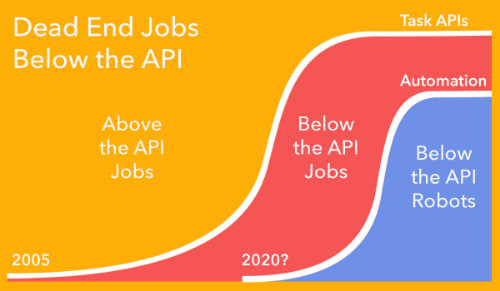
\includegraphics[scale=.5]{aboveapi.png}
\end{figure}
As our world becomes more complex, the design thinking movement in education and in industry hopes to democratize the innovation process so that more people are endowed with the skills to solve hard problems. Design thinking was developed by IDEO founder David Kelley; it's essentially a set of mindsets and processes to develop human-centered, innovative solutions \cite{forbesdt}. Developing empathy for the user is a core component of the process, as is rapid prototyping and feedback-driven iteration.\par
The engineering design process is very similar to the mindsets of design thinking: define the problem, brainstorm solutions, test, and iterate. One of the differences is that engineering does not always emphasize a human-centered design approach. As an example, designing a robotic system to land on an asteroid involves constant prototyping, testing, and iteration, but the human perspective may not be as relevant. Nevertheless, design thinking is highly useful to many engineering projects, and engineering is an important discipline in innovation and problem-solving. \par
In the age of rapid change, the ability to innovate may be a more pressing educational objective than instilling foundational computational thinking CS concepts. Fortunately, CS is one of the most powerful platforms for innovation, and so meeting both learning objectives simultaneously is both possible and potentially advantageous. CS affords the ability to rapidly prototype, perform virtual testing, and continually iterate---pillars of the design thinking process. CS can be used to program hardware (wearable technology, robotics, self-driving cars, 3D printers, etc.) and software solutions (mobile devices, web applications, music, financial data, math, etc.). In short, the possibilities are endless, and CS is an incredible tool to solve some of the world's most difficult challenges.\par
The obvious examples of software companies that have dramatically changed our daily lives include companies like Uber, AirBnB, Google, Facebook, and Amazon. But there are innumerable examples of innovation through code with altruistic and humanitarian origins. Ushahidi, an open source crowd-sourcing platform to report crisis information during earthquakes or humanitarian disasters, is one example. The project was originally developed to map reports of violence in Kenya after the post-election violence in 2008 \cite{ushahidi} and has also been used by the Louisiana Bucket Brigade to map the human and environmental impacts of oil spills \cite{labb}. Myo armband, an incredibly versatile wireless wearable technology that tracks arm gestures and motion, may help deaf people communicate by turning sign language into text \cite{myowhat}. \par 
Massachusetts Institute of Technology's (MIT) Media Lab is one of the best examples of an integrated, ``antidisciplinary" approach to innovation that employs design, engineering, and computer science as tools to develop game-changing technology in myriad fields. Fab labs---spaces with woodworking equipment, laser cutters, 3D printers, electronics, and other shop tools---abound throughout the graduate school, giving students ample access to tools necessary to prototype and develop creative projects. From the MIT website:
\begin{blockquote}
	``Actively promoting a unique, antidisciplinary culture, the MIT Media Lab goes beyond known boundaries and disciplines, encouraging the most unconventional mixing and matching of seemingly disparate research areas. It creates disruptive technologies that happen at the edges, pioneering such areas as wearable computing, tangible interfaces, and affective computing. Today, faculty members, research staff, and students at the Lab work in 24 research groups on more than 350 projects that range from digital approaches for treating neurological disorders, to a stackable, electric car for sustainable cities, to advanced imaging technologies that can “see around a corner.” The Lab is committed to looking beyond the obvious to ask the questions not yet asked–questions whose answers could radically improve the way people live, learn, express themselves, work, and play" \cite{mitmediaabout}.
	\end{blockquote}
A tour of the building in April, 2016 revealed that every research group was using CS in some way. The Center for Lifelong Kindergarten is a multidisciplinary group developing solutions to engage people in creative learning experiences. This group is responsible for creative coding platforms like Scratch, App Inventor, LEGO Mindstorms, and the Makey Makey. In the Center for Bits and Atoms (CBA), an ``initiative exploring the boundary between computer science and physical science'' that ``studies how to turn data into things, and things into data'' \cite{cba}, a graduate student is currently developing a 3D world for simulating nano-scale electronic structures using JavaScript and Three.js. In the Synthetic Neurobiology group, researchers are attempting to repair brain disorders ``via novel tools for mapping and fixing brain computations" \cite{synth}. There are many more examples of the creative application of code used in Media Lab to break the boundaries of what is currently feasible and continually innovate. \par
The Maker Movement has the potential to wrap all of these disciplines---CS, engineering, design thinking---into a single pedagogical approach that teaches and encourages innovation through hands-on, project-based learning. The Maker Movement was spawned by the emergence of new, easy-to-learn tools like 3D printers, laser cutters, and programmable electronics, tools that are democratizing innovation. Arduinos and Raspberry Pis, simple programmable computers, are making complex electronics projects accessible to tinkerers of all types. Artists, technophiles, programmers, machinists, and DIY-enthusiasts are converging in ``makerspaces'' to create, share, and invent, while online platforms like \href{http://instructables.com}{Instructables.com} allow makers to virtually share step-by-step tutorials for drones, electronic music instruments, 3D printed bobble heads, and more.\par
Education is increasingly buying in to the Maker Movement. Newman, Patrick F. Taylor, McGehee School, and Lusher High School are just a few examples of schools in New Orleans that are including making in the curriculum. Many schools have already recognized the power of hands-on, experiential learning, an approach backed by research. A study from Purdue showed that students scored higher in science classes where the goal was to design and build a device than students in traditional classrooms \cite{purdue}. A study from the University of Chicago had similar findings; brain scans revealed that students' sensory and motor-related brain regions were activated when they thought about topics like angular momentum and torque \cite{uchic}. Making allows students to chart their own paths, to choose their own hard problems, and to actively engage in the exploration of electronics, programming, and art.\par  
By refocusing the educational learning objective from the need to instill computational thinking mindsets to the need to foster creative and innovative thinking skills, integrating CS into design thinking, engineering, and the Maker Movement makes sense. Computer science is an incredibly versatile tool, and using this tool to solve human-centered or open-ended design challenges may be the most effective, valuable, and necessary approach to CS education. \par
% When asked about the role of computer science in K-12 education, Malis responded: ``Our job is to prepare students. If our students graduate without any exposure to coding, we aren't doing our job."
